\apendice{Documentación de usuario}

\section{Introducción}
Esta sección se centra en la explicación y demostración de cómo se debe utilizar la aplicación, de forma intuitiva y sencilla.
\section{Requisitos de usuarios}
Para que un usuario pueda ejecutar y usar nuestra aplicación, deberá tener instalado Python 3.5 en su máquina, aunque para facilitar al usuario no tener que saber como descargar las librerías o dependencias, hemos implementado un script que funcionará teniendo instalado Miniconda para Python 3.5, explicaremos su uso en la instalación.

\begin{itemize}
	\item Tener una distribución Windows instalada.

	\item Python 3.5: Para poder ejecutar necesitaremos tener Python 3.5.
	\begin{itemize}
		\item Miniconda para Python 3.5:
		
		Se puede descargar a través del siguiente enlace \url{http://conda.pydata.org/miniconda.html} y siguiendo las instrucciones a traves de este otro enlace \url{http://conda.pydata.org/docs/install/quick.html#windows-miniconda-install}.		
		
		Es una distribución que incluye Python y facilita el uso de este lenguaje y la instalación de multitud de librerías.
		
		Sera necesario tenerlo instalado en la carpeta principal de nuestro usuario \textrm{C:\textbackslash Users\textbackslash NombreTuUsuario}
	\end{itemize}
	
	\item Tener el proyecto descargado o clonado con los fuentes:
	
	Se puede descargar a través del siguiente enlace \url{https://github.com/Itg0001/TFG_DietaPorDientes.git}

\end{itemize}

\section{Instalación}

Una vez que tengamos Miniconda para Python 3.5 y el proyecto descargado o clonado, podremos proceder a la instalación del mismo, siguiendo los pasos descritos a continuación:

\begin{itemize}
	\item Primero, si hemos descargado el proyecto lo tendremos en formato .zip deberemos descomprimirlo en la carpeta deseada.
	
	\item Una vez descomprimido dentro del directorio del proyecto estará ubicado un ejecutable para Windows .bat llamado <<\textrm{EjecutarGui.bat}>>.
	
	Procederemos a hacer doble clic sobre este fichero ejecutable y se abrirá una terminal, la primera vez que lo hagamos, tardará un rato, porque descarga las librerías necesarias para la ejecución del mismo.
	
	\item Una vez terminado el proceso anterior, se abrirá la aplicación.
\end{itemize}

\subsection{Posibles errores}
En caso de que al instalar o descargar los paquetes salte algún error esto, puede deberse a que se ha perdido la conexión a Internet y no puede descargar los paquetes necesarios.
Para solucionarlo volvemos a ejecutar y comenzará donde se quedó al caerse la red. No perdemos el tiempo usado hasta ese momento.

Otro fallo común es que no se haya instalado la distribución de Miniconda sobre el directorio indicado: \textrm{C:\textbackslash Users\textbackslash NombreTuUsuario}.
Para solucionar este problema deberemos instalarlo sobre este directorio.

En caso de que surja algún otro problema contactar con el desarrollador a través del siguiente e-mail: \textrm{itg0001\makeatletter @ alu.ubu.es}

\section{Manual del usuario}

Una vez tengamos todo bien configurado y la aplicación se ejecute correctamente, deberíamos tener esta ventana inicial, como se ve en la figura \ref{fig:E.1}.

\begin{figure}[h]
\centering
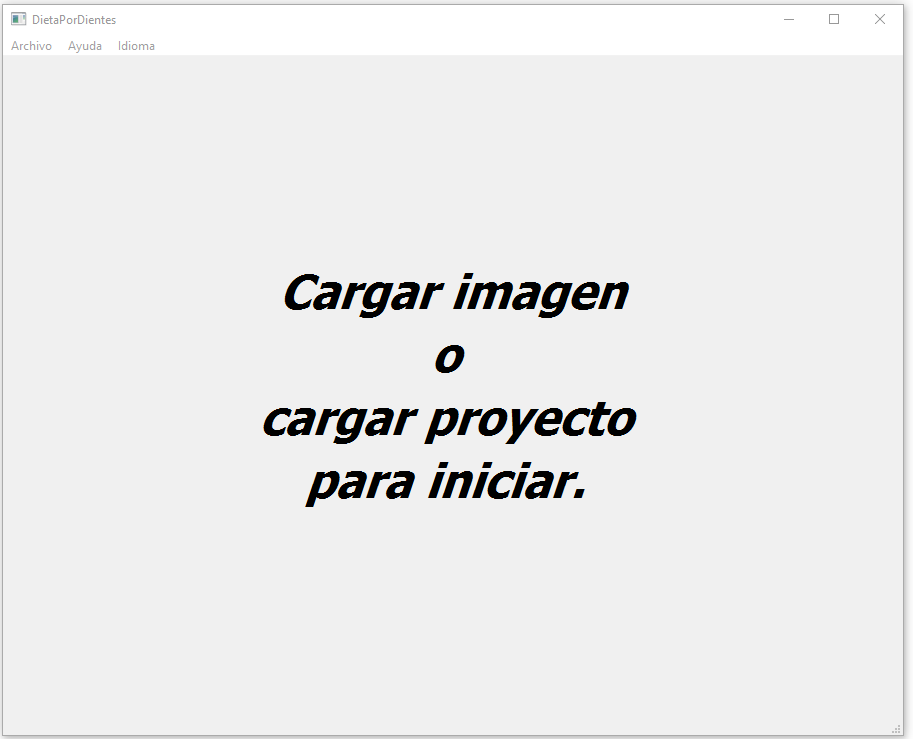
\includegraphics[width=.99\textwidth]{VentanaInicial}
\caption{Ventana inicial de la aplicación}
\label{fig:E.1}
\end{figure}
Una vez llegados a este punto tendremos varias opciones para editar o calculas las estrías de una imagen, dependiendo, si la imagen esta en blanco o si las estrías ya están pintadas sobre ella, tendremos las siguientes opciones:

\begin{itemize}
	\item Abrir imagen \ref{modo:1}:
	\item Cargar proyecto \ref{modo:2}:
\end{itemize}

\subsection{Abrir imagen}
\label{modo:1}

En esta sección se explicará como cargar una imagen en nuestra aplicación, para empezar un proyecto desde cero.

Deberemos seleccionar la opción de Archivo  $>$ Nuevo Proyecto. Como se puede ver en la imagen \ref{fig:abrirPro}

Un proyecto estará compuesto por:
\begin{itemize}
\item Original.jpg: Se corresponde con la imagen original antes de detectar o pintar estrías sobre ella.
\item Pintada.jpg: Se corresponde con la imagen resultante con las estrías detectadas pintadas sobre ella.
\item Proyecto.xml: Este fichero contendrá la configuración del proyecto y los valores que hemos asignado para los cálculos de nuestra ejecución.
\item Salida Estadísticas.csv: Este fichero contendrá las estadísticas de las estrías que hemos detectado medias, desviación típica y calculo del punto en las elipses de dieta.
\item Salida Lineas.csv: Este fichero contendrá la información de longitud, ángulo, inicio y final de cada una de las estrías detectadas.
\item Tabla.tex: Este fichero contendrá la tabla para exportar a documentos latex y crear informes con las estadísticas de las estrías detectadas.
\end{itemize}

\begin{figure}[h]
\centering
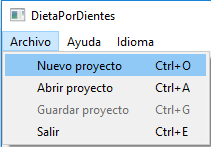
\includegraphics[width=.50\textwidth]{AbrirImagen}
\caption{Opción para cargar una imagen}
\label{fig:abrirPro}
\end{figure}

Una vez que hagamos click en este punto, se nos muestra una ventana para elegir ficheros, en el cual debemos explorar hasta la carpeta donde estén las imágenes que queremos analizar. Como podemos observar en la figura \ref{fig:abrirPaso2}

\begin{figure}[h]
\centering
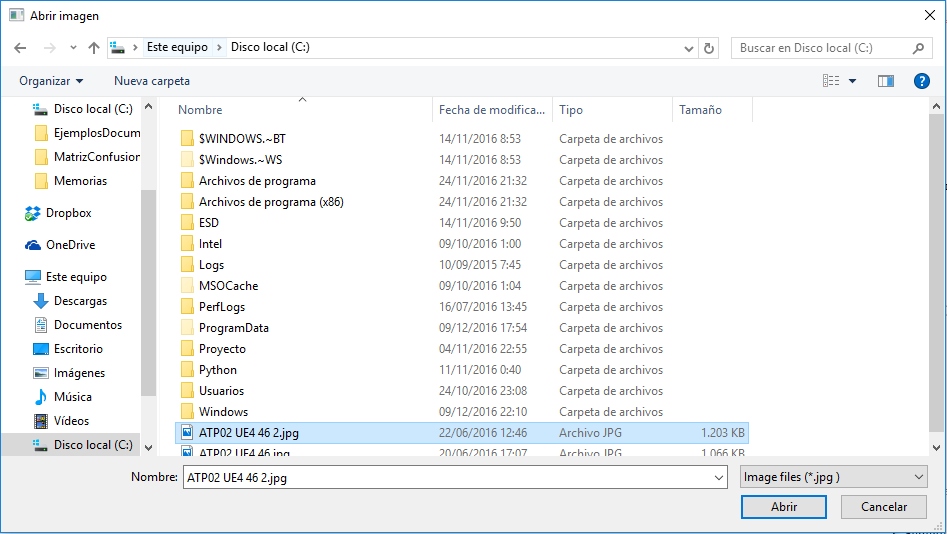
\includegraphics[width=.99\textwidth]{AbrirPaso2}
\caption{Seleccionador de ficheros}
\label{fig:abrirPaso2}
\end{figure}

Una vez seleccionado deberemos dar a aceptar si hemos seleccionado la imagen que queremos evaluar.
Dependiendo de la imagen que hemos abierto pueden pasar dos cosas: uno \ref{fig:opcion1}, que la imagen abierta este pintada, dos \ref{fig:opcion2}, que la imagen abierta no este pintada. Dependiendo de esto tendremos estas dos ventanas, como se muestra en la figura \ref{fig:figuraTipos}.


\begin{figure}
	\begin{subfigure}[c]{.55\linewidth}
	\centering\large 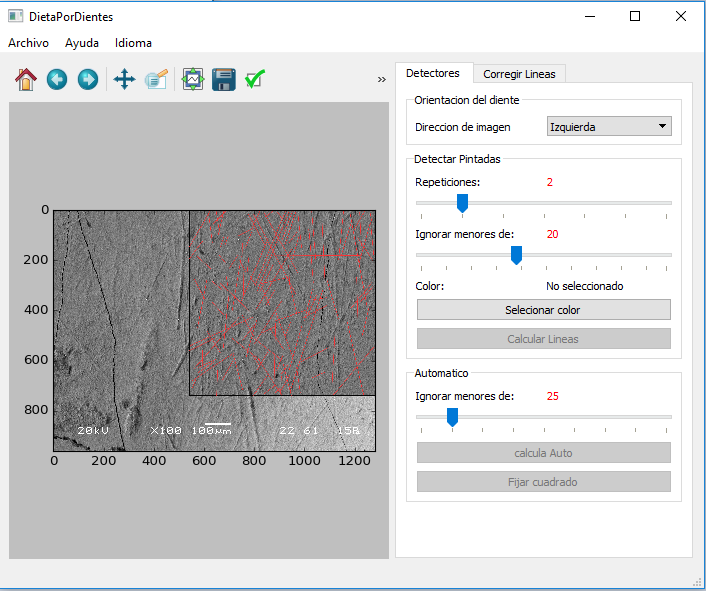
\includegraphics[width=.9\textwidth]{opcion1}
	\caption{Opción con lineas pintadas.}\label{fig:opcion1}
	\end{subfigure}%
	\begin{subfigure}[c]{.55\linewidth}
	\centering\large 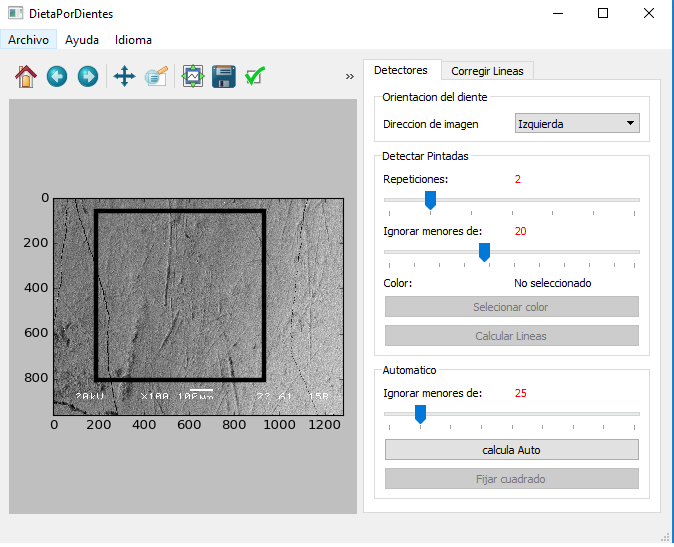
\includegraphics[width=.9\textwidth]{opcion2}
	\caption{Opción con lineas sin pintar.}\label{fig:opcion2}
	\end{subfigure}%
	\label{fig:figuraTipos}
	\caption{Opciones de apertura de imagen.}
\end{figure}




\subsection{Cargar proyecto}
\label{modo:2}

En esta sección se explicará como cargar un proyecto en nuestra aplicación, para continuar un proyecto ya empezado.

Deberemos seleccionar la opción de Archivo  $>$ Abrir Proyecto. Como se puede ver en la figura \ref{fig:cargarPro}


\begin{figure}[h]
\centering
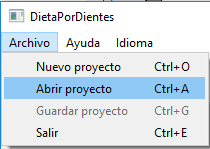
\includegraphics[width=.50\textwidth]{CargarProyecto}
\caption{Opción para abrir un proyecto.}
\label{fig:cargarPro}
\end{figure}

Una vez que hacemos clic sobre la opción de abrir proyecto, ahora debemos explorar, como podemos observar en la siguiente figura \ref{fig:selecCargarPro}, hasta el directorio que contiene los ficheros que se generan al guardar un proyecto \textrm{<<Pintada.jpg, Original.jpg, Proyecto.xml, Salida-Estadisticas.csv, Salida-Lineas.csv y Tabla.tex>>}  y una vez seleccionado el directorio que contiene los ficheros del proyecto, damos a \textrm{<<Abrir carpeta>>} para cargar el proyecto. 



\begin{figure}[h]
\centering
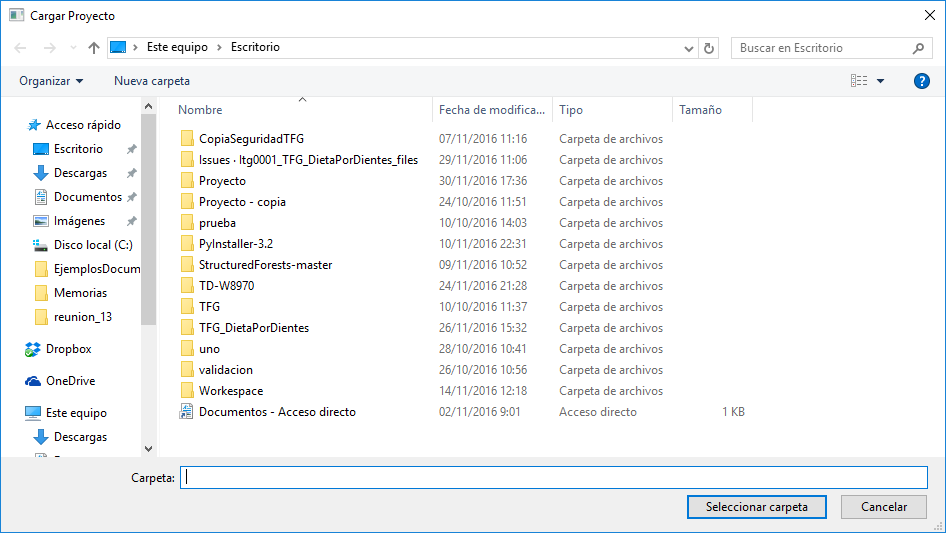
\includegraphics[width=.99\textwidth]{selecCargarPro}
\caption{Opción para abrir un proyecto.}
\label{fig:selecCargarPro}
\end{figure}

Una vez abierto el proyecto tendremos la imagen junto con sus estrías guardadas que estarán pintadas sobre la imagen, como podemos observar en la figura \ref{fig:proyectoAbierto}.


\begin{figure}[h]
\centering
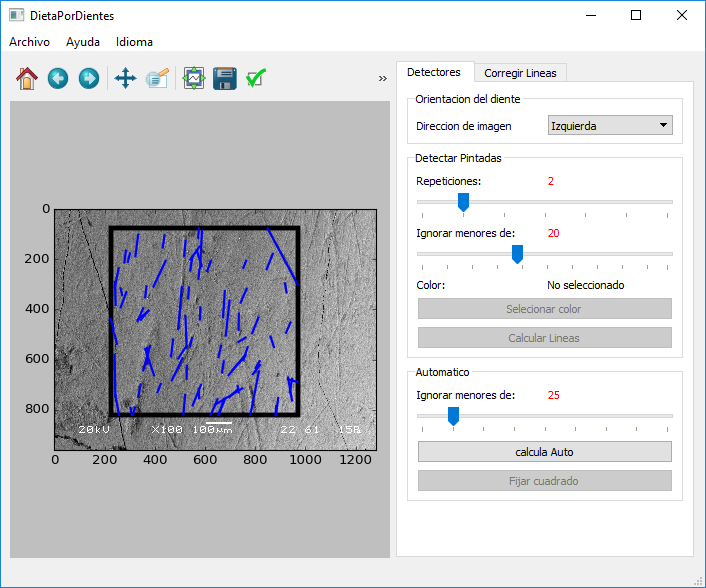
\includegraphics[width=.99\textwidth]{proyectoAbierto}
\caption{Como se muestra un proyecto cargado o abierto.}
\label{fig:proyectoAbierto}
\end{figure}

\subsection{Cambiar idioma}
\label{modo:idioma}

Para cambiar el idioma de la aplicación, deberemos seleccionar en el menú principal, <<Idioma $>$ Una de las dos opciones>> como podemos observar en la figura \ref{fig:camb}.

Hemos optado por cambiar el idioma de la aplicación para que perduren los cambios en futuras ejecuciones, para realizar esto, debemos reiniciar la aplicación. Si tenemos datos sin guardar, nos preguntará si queremos guardar los cambios o no antes de cerrar la aplicación.

\begin{figure}[h]
\centering
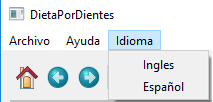
\includegraphics[width=.55\textwidth]{CambiarIdioma}
\caption{Como cambiar el idioma.}
\label{fig:camb}
\end{figure}

\subsection{Modo semi-automático para lineas pintadas}

Este modo solamente podrá ser usado cuando dispongamos de una imagen que tenga las estrías pintadas sobre ella y estas estén contenidas dentro de un cuadrado que delimite su área, como podemos observar en la figura \ref{fig:semiAutoCorrecto}.



\begin{figure}[h]
\centering
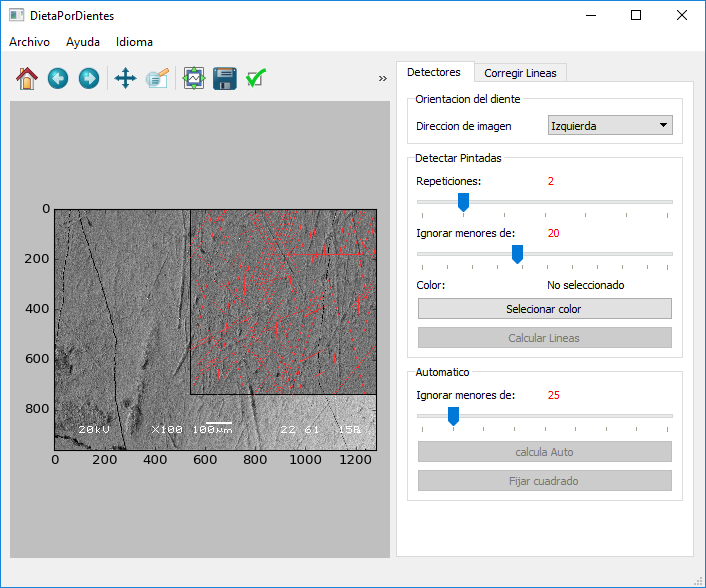
\includegraphics[width=.99\textwidth]{semiAutoCorrecto}
\caption{Imagen válida para detección de estrías modo semiautomático.}
\label{fig:semiAutoCorrecto}
\end{figure}

Una vez que tengamos una imagen con las estrías pintadas cargada y válida como mostramos en la figura, procederemos a seleccionar su orientación, como muestra en la figura \ref{fig:selOrientacion}.

\begin{figure}[h]
\centering
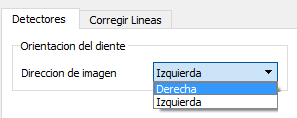
\includegraphics[width=.55\textwidth]{selOrientacion}
\caption{Selección de la orientación de la imagen.}
\label{fig:selOrientacion}
\end{figure}

A continuación deberemos seleccionar tanto el número de repeticiones del algoritmo para la obtención de los segmentos pintados <<Cuanto mayor número de ellos mas tiempo tardara>>, la longitud mínima que debe ignorar el algoritmo para no detectar segmentos muy pequeños. Como podemos observar en la figura \ref{fig:opcionesAlg}.

\begin{figure}[h]
\centering
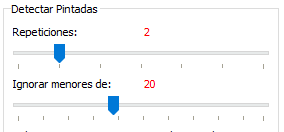
\includegraphics[width=.55\textwidth]{opcionesAlg}
\caption{Selección de las opciones disponibles para este modo.}
\label{fig:opcionesAlg}
\end{figure}

Finalmente, nos quedaría la opción mas importante que sin ella el algoritmo no podrá ser ejecutado. Es seleccionar el color del que estén pintadas las lineas, para ello deberemos hacer click sobre el botón <<Seleccionar color>>, como podemos observar en la figura \ref{fig:selecionarColorP1} y después de hacer click sobre el, este se desactivará, como podemos observar en la figura \ref{fig:selecionarColorP2}.
Las estrías pintadas a veces pueden ser muy finas y no seremos capaces de clicar sobre esos pixeles, por lo que en este caso deberemos ampliar la imagen en una región que contenga estrías pintadas. Para ampliar debemos seleccionar el botón de ampliar y dibujar un rectángulo sobre la imagen con el clic derecho pulsado, como podemos observar en la figura \ref{fig:selecionarColorP3}.
Una vez seleccionado el color correctamente, cuando este pintado el label de color actual con el color de las estrías pintadas, se activará el botón de calcular las lineas, como podemos observar en la figura \ref{fig:selecionarColorP4}.



\begin{figure}
	\begin{subfigure}[c]{.5\linewidth}
	\centering\large 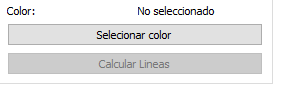
\includegraphics[width=.9\textwidth]{selecionarColorP1}
	\caption{Selección del color en el que estén las estrías pintadas.}\label{fig:selecionarColorP1}
	\end{subfigure}%
	\begin{subfigure}[c]{.5\linewidth}
	\centering\large 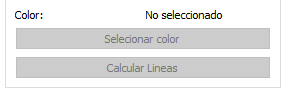
\includegraphics[width=.9\textwidth]{selecionarColorP2}
	\caption{Después de hacer click sobre él.}
	\label{fig:selecionarColorP2}
	\end{subfigure}%
	
	\begin{subfigure}[c]{.5\linewidth}
	\centering\large 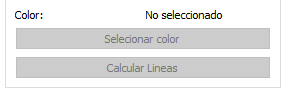
\includegraphics[width=.9\textwidth]{selecionarColorP2}
	\caption{Ampliar región.}
	\label{fig:selecionarColorP3}
	\end{subfigure}%
	\begin{subfigure}[c]{.5\linewidth}
	\centering\large 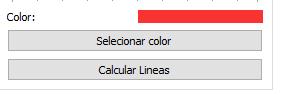
\includegraphics[width=.9\textwidth]{selecionarColorP4}
	\caption{Después de seleccionar correctamente el color.}
	\label{fig:selecionarColorP4}
	\end{subfigure}%
	\label{fig:pasosColor}
	\caption{Pasos para seleccionar el color correctamente.}
\end{figure}

Para finalizar, una vez que hagamos click en el botón de calcular lineas ya podremos añadir estrías nuevas, eliminar algunos segmentos, borrar todos o guardar los datos del proyecto para calcular las estadísticas de las estrías.


\subsection{Modo manual}
Después de cargar una imagen. Ya sea pintada o sin pintar. Deberemos abrir una imagen como indica el apartado \ref{modo:1} o abrir un proyecto tal y como indican el apartado \ref{modo:2}.
Una vez que tengamos la imagen o el proyecto cargado podremos pintar nuevas estrías en la imagen siguiendo los siguientes pasos.

\begin{itemize}
\item Pulsaremos el botón de corregir lineas, como muestra la figura \ref{fig:CorregirPaso1}.

\item Una vez pulsado deberemos seleccionar dos puntos: inicio y final del segmento que queremos añadir. 
Dentro del recuadro de la región pintable que esta delimitada por un recuadro negro, como se muestra en las figuras \ref{fig:punto1} y \ref{fig:punto2}, ahora solo nos quedara añadir el segmento a la tabla como muestra la figura \ref{fig:anadirsegment}.
\end{itemize}

\begin{figure}
	\begin{subfigure}[c]{.5\linewidth}
	\centering\large 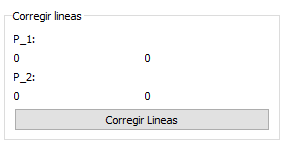
\includegraphics[width=.9\textwidth]{CorregirPaso1}
	\caption{Activar el modo de corregir o añadir un segmento.}\label{fig:CorregirPaso1}
	\end{subfigure}%
	\begin{subfigure}[c]{.5\linewidth}
	\centering\large 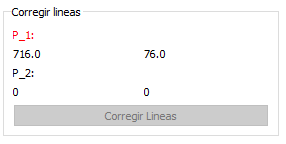
\includegraphics[width=.9\textwidth]{punto1}
	\caption{Primer punto seleccionado.}\label{fig:punto1}
	\end{subfigure}%
	
	\begin{subfigure}[c]{.5\linewidth}
	\centering\large 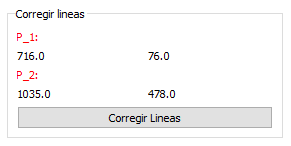
\includegraphics[width=.9\textwidth]{punto2}
	\caption{Segundo punto seleccionado.}\label{fig:punto2}
	\end{subfigure}%
	\begin{subfigure}[c]{.5\linewidth}
	\centering\large 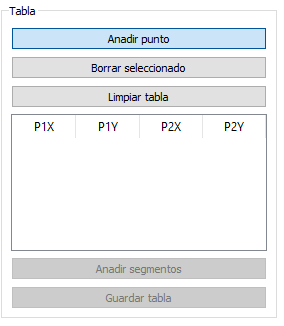
\includegraphics[width=.9\textwidth]{anadirsegment}
	\caption{Añadir segmento.}\label{fig:anadirsegment}
	\end{subfigure}%
	\caption{Pasos para añadir un segmentos manualmente.}
\end{figure}

	
Para los demás pasos no hace falta explicación ya que sus respectivos botones dicen claramente que funciones desempeñan.	
	
\subsection{Modo automático}
Después de cargar una imagen sin pintar deberemos abrir una imagen como indica el apartado \ref{modo:1} o abrir un proyecto tal y como indica el apartado \ref{modo:2}.

Una vez que tengamos la imagen o el proyecto cargado, podremos configurar el modo automático, lo primero será asignar la orientación de la imagen, como podemos ver en la figura \ref{fig:selOrientacion}, también deberemos seleccionar la longitud mínima de corte que ignorará el algoritmo automático, como podemos observar en la figura \ref{fig:selTam}.

\begin{figure}[h]
\centering
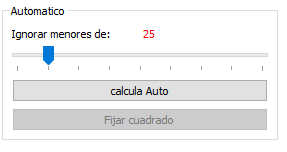
\includegraphics[width=.55\textwidth]{selTam}
\caption{Selección de la longitud mínima de corte.}
\label{fig:selTam}
\end{figure}

Una vez seleccionado el tamaño mínimo de corte podremos ejecutar el algoritmo haremos click sobre el botón de calcular automático, obteniendo el resultado mostrado en la figura \ref{fig:CalculadasAuto} y podremos mover el recuadro del área con el que nos queremos quedar a la región de interés que consideremos apropiada.

\begin{figure}[h]
\centering
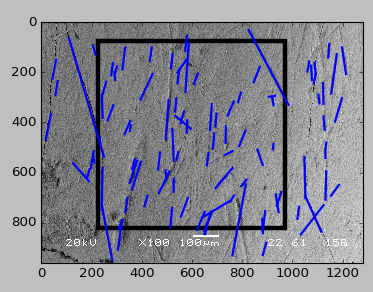
\includegraphics[width=.9\textwidth]{CalculadasAuto}
\caption{Segmentos calculados por el modo automático.}
\label{fig:CalculadasAuto}
\end{figure}

Una vez que la situemos donde mayor densidad de estrías haya detectado, la fijaremos e ignorará las que se queden por fuera de la región, como podemos observar en la figura \ref{fig:automati}.

\begin{figure}[h]
\centering
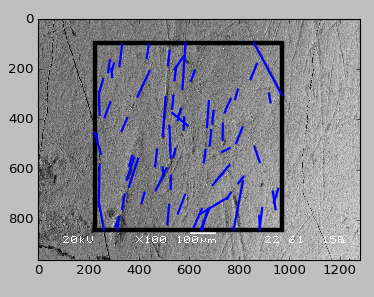
\includegraphics[width=.9\textwidth]{automati}
\caption{Segmentos englobados en el cuadrado.}
\label{fig:automati}
\end{figure}

Pasado este punto, en la pestaña de corregir lineas quedarán añadidas todas aquellas que ha detectado el algoritmo y hemos encuadrado en la región factible, de estas lineas podremos obtener tanto estadísticas como un proyecto para editar mas adelante. Guardando el proyecto con el botón para dicha función.

\subsection{Guardar proyecto}

En este apartado vamos a explicar como guardar un proyecto una vez que hayamos abierto o cargado una imagen, calculado las estrías con el modo semiautomático o por el automático, y la tabla este rellenada con estas. 
Si el proyecto es cargado a partir de uno ya existente, no tener abiertas las estadísticas en Excel o cualquier otro editor, porque sino no funcionará la operación de guardar. Esto sera transparente al usuario porque dejara los ficheros como estaban antes, no los modificará, e informará al usuario de que no han sido guardados. 

Podemos usar tanto el botón de guardar que aparece en la pestaña dos, la pestaña de corregir lineas, \ref{fig:BotonGuarPesta} como el botón del menú principal que aparece en la figura \ref{fig:BotonGuar}

\begin{figure}
	\begin{subfigure}[c]{.5\linewidth}
	\centering\large 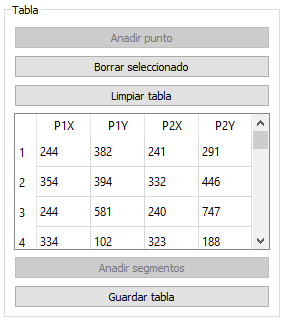
\includegraphics[width=.9\textwidth]{BotonGuarPesta}
	\caption{Boton de guardar en la pestaña, corregir lineas.}\label{fig:BotonGuarPesta}
	\end{subfigure}%
	\begin{subfigure}[c]{.5\linewidth}
	\centering\large 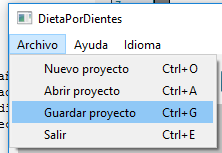
\includegraphics[width=.9\textwidth]{BotonGuar}
	\caption{Boton de guardar en el menu principal.}\label{fig:BotonGuar}
	\end{subfigure}%
	\caption{Opciones para guardar tabla.}
\end{figure}
